\chapter{Implementacija i korisničko sučelje}
		
		
		\section{Korištene tehnologije i alati}
		
			 Komunikacija među članovima projektnog tima ostvarena je pomoću platforme  \underline{Microsoft Teams} \footnote{https://www.microsoft.com/en-us/microsoft-365/microsoft-teams/group-chat-software} preko koje su održavani video sastanci te pomoću mobilne aplikacije za razmjenu poruka \underline{WhatsApp}  \footnote{https://www.whatsapp.com}. Za pisanje dokumentacije korišten je programski jezik za dokumente \underline{LaTeX} \footnote{https://www.latex-project.org/} i LaTeX uređivač \underline{Texstudio} \footnote{https://www.texstudio.org/}, za izradu različitih UML dijagrama korišten je alat \underline{Astah UML} \footnote{https://astah.net/products/astah-community/}, dok je za izradu ER dijagrama baze podataka korišten alat za baze podataka \underline{DBeaver} \footnote{https://dbeaver.io/}. Za upravljanje inačicama datoteka projekta korišten je distribuirani sustav \underline{Git} \footnote{https://git-scm.com/}, a repozitorij projektne grupe uspostavljen je na \underline{GitLabu} \footnote{https://about.gitlab.com/}. GitLab je web hosting usluga koja podržava rad sustava Git.
			 
			 Za razvojno okruženje korišten je \underline{IntelliJ IDEA} \footnote{https://www.jetbrains.com/idea/}, integrirano razvojno okruženje (IDE) koje je razvila tvrtka JetBrains. Ponajviše je namijenjeno za Javu, no podržava i mnogo drugih programskih jezika kao što su Kotlin, Scala, Python i drugi. Koristi se za razvoj, modeliranje i \textit{deployment} web i mobilnih aplikacija. 
			 
			 Za izradu web aplikacije korišten je radni okvir \underline{Spring Boot} \footnote{https://spring.io/projects/spring-boot}. Spring Boot je specijalizacija radnog okvira Spring a omogućuje jednostavnije i brže oblikovanje web aplikacija tako što u svojoj automatskoj konfiguraciji više uobičajenih dijelova web aplikacije već ima podešeno. Od programskih jezika koriste se objektno orijentirani jezik \underline{Java} \footnote{https://www.java.com/en/} za izradu \textit{backend} sloja aplikacije  skriptni programski jezik \underline{JavaScript} \footnote{https://www.javascript.com/} te knjižnica \underline{React} \footnote{https://reactjs.org/}  za izradu \textit{frontend} sloja. Knjižnicu React razvija tvrtka Facebook a pisana je u jeziku JavaScript i sadrži mnogo paketa te je tako fleksibilna za različite aplikacije. 
			 
			 Baza podataka nalazi se na javno dostupnom poslužitelju \underline{Heroku} \footnote{https://www.heroku.com/}.
			
			
			\eject 
		
	
		\section{Ispitivanje programskog rješenja}
			
			\textbf{\textit{dio 2. revizije}}\\
			
			 \textit{U ovom poglavlju je potrebno opisati provedbu ispitivanja implementiranih funkcionalnosti na razini komponenti i na razini cijelog sustava s prikazom odabranih ispitnih slučajeva. Studenti trebaju ispitati temeljnu funkcionalnost i rubne uvjete.}
	
			
			\subsection{Ispitivanje komponenti}
			\textit{Potrebno je provesti ispitivanje jedinica (engl. unit testing) nad razredima koji implementiraju temeljne funkcionalnosti. Razraditi \textbf{minimalno 6 ispitnih slučajeva} u kojima će se ispitati redovni slučajevi, rubni uvjeti te izazivanje pogreške (engl. exception throwing). Poželjno je stvoriti i ispitni slučaj koji koristi funkcionalnosti koje nisu implementirane. Potrebno je priložiti izvorni kôd svih ispitnih slučajeva te prikaz rezultata izvođenja ispita u razvojnom okruženju (prolaz/pad ispita). }
			
			
			
			\subsection{Ispitivanje sustava}
			
			 \textit{Potrebno je provesti i opisati ispitivanje sustava koristeći radni okvir Selenium\footnote{\url{https://www.seleniumhq.org/}}. Razraditi \textbf{minimalno 4 ispitna slučaja} u kojima će se ispitati redovni slučajevi, rubni uvjeti te poziv funkcionalnosti koja nije implementirana/izaziva pogrešku kako bi se vidjelo na koji način sustav reagira kada nešto nije u potpunosti ostvareno. Ispitni slučaj se treba sastojati od ulaza (npr. korisničko ime i lozinka), očekivanog izlaza ili rezultata, koraka ispitivanja i dobivenog izlaza ili rezultata.\\ }
			 
			 \textit{Izradu ispitnih slučajeva pomoću radnog okvira Selenium moguće je provesti pomoću jednog od sljedeća dva alata:}
			 \begin{itemize}
			 	\item \textit{dodatak za preglednik \textbf{Selenium IDE} - snimanje korisnikovih akcija radi automatskog ponavljanja ispita	}
			 	\item \textit{\textbf{Selenium WebDriver} - podrška za pisanje ispita u jezicima Java, C\#, PHP koristeći posebno programsko sučelje.}
			 \end{itemize}
		 	\textit{Detalji o korištenju alata Selenium bit će prikazani na posebnom predavanju tijekom semestra.}
			
			\eject 
		
		
		\section{Dijagram razmještaja}
		
			Dijagram razmještaja statički je UML dijagram koji prikazuje i opisuje topologiju sustava te programsku potporu za implementaciju sustava. Korisnik, to jest klijent na svom osobnom računalu koristi web preglednik za pristup web aplikaciji. Na poslužiteljskom računalu nalazi se Tomcat web poslužitelj te PostgreSQL poslužitelj baze podataka. Komunikacija između klijenta i poslužitelja odvija se preko protokola aplikacijskog sloja HTTP.
			
			\begin{figure}[H]
				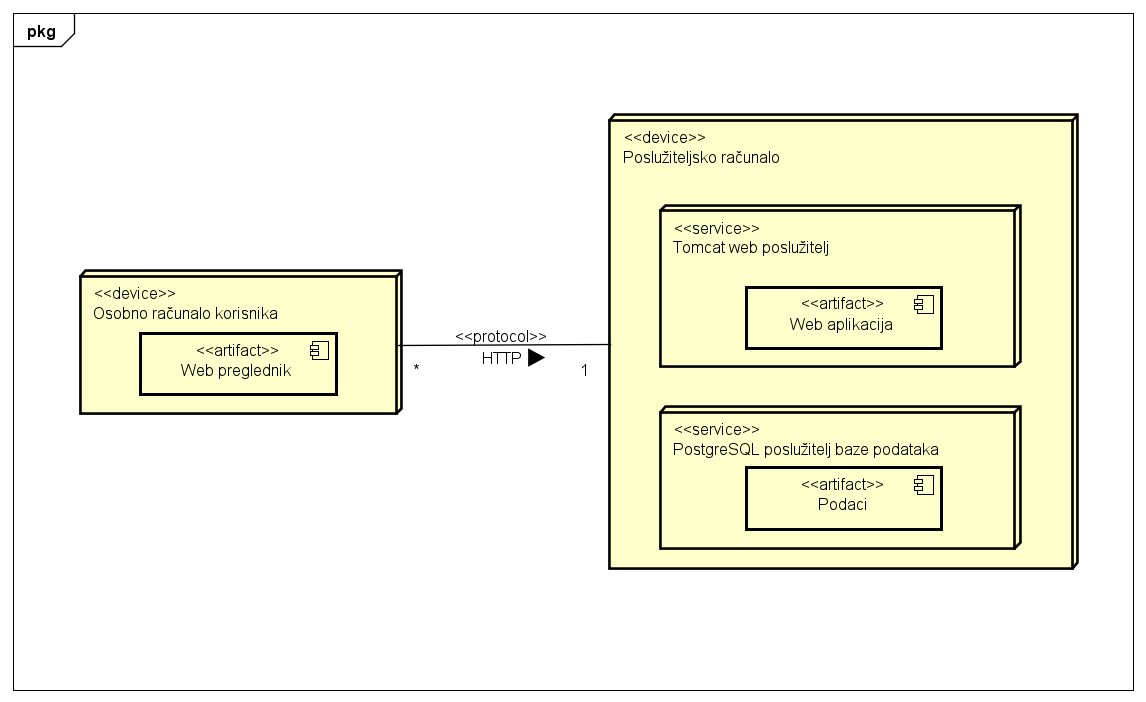
\includegraphics[scale=0.5]{dijagrami/DeployDiagram} %veličina slike u odnosu na originalnu datoteku i pozicija slike
				\centering
				\caption{Dijagram razmještaja}
				\label{fig:dijagramRazmjestaja}
			\end{figure}
			
			 
			\eject 
		
		\section{Upute za puštanje u pogon}
		
			\textbf{\textit{dio 2. revizije}}\\
		
			 \textit{U ovom poglavlju potrebno je dati upute za puštanje u pogon (engl. deployment) ostvarene aplikacije. Na primjer, za web aplikacije, opisati postupak kojim se od izvornog kôda dolazi do potpuno postavljene baze podataka i poslužitelja koji odgovara na upite korisnika. Za mobilnu aplikaciju, postupak kojim se aplikacija izgradi, te postavi na neku od trgovina. Za stolnu (engl. desktop) aplikaciju, postupak kojim se aplikacija instalira na računalo. Ukoliko mobilne i stolne aplikacije komuniciraju s poslužiteljem i/ili bazom podataka, opisati i postupak njihovog postavljanja. Pri izradi uputa preporučuje se \textbf{naglasiti korake instalacije uporabom natuknica} te koristiti što je više moguće \textbf{slike ekrana} (engl. screenshots) kako bi upute bile jasne i jednostavne za slijediti.}
			
			
			 \textit{Dovršenu aplikaciju potrebno je pokrenuti na javno dostupnom poslužitelju. Studentima se preporuča korištenje neke od sljedećih besplatnih usluga: \href{https://aws.amazon.com/}{Amazon AWS}, \href{https://azure.microsoft.com/en-us/}{Microsoft Azure} ili \href{https://www.heroku.com/}{Heroku}. Mobilne aplikacije trebaju biti objavljene na F-Droid, Google Play ili Amazon App trgovini.}
			
			
			\eject 
